\documentclass[xcolor=dvipsnames, notes=hide]{beamer}
%\documentclass[xcolor=dvipsnames, notes=only]{beamer}
%\documentclass[xcolor=dvipsnames]{beamer}
%\setbeameroption{show only notes}
%\usepackage{pgfpages}
%\setbeamertemplate{note page}[plain]
%\setbeameroption{show notes on second screen=right}

\usepackage[english]{babel}
\usepackage[utf8]{inputenc}
\usepackage[T1]{fontenc} % Ligaturen, richtige Umlaute im PDF

\newcommand{\IR}{\mathbb{R}}
\newcommand{\backupbegin}{
	\newcounter{finalframe}
	\setcounter{finalframe}{\value{framenumber}}
}
\newcommand{\backupend}{
	\setcounter{framenumber}{\value{finalframe}}
}

\usepackage[absolute,overlay]{textpos} % textblock for figure placement

\usepackage{tabularx, booktabs}
\usepackage{amsmath}
\usepackage{blkarray, bigstrut}
\usepackage{xparse}

\usepackage[normalem]{ulem} % for \sout{}
\usepackage[ruled]{algorithm}
\usepackage{algpseudocode} 
\makeatletter
\def\BState{\State\hskip-\ALG@thistlm}
\algdef{SE}[DOWHILE]{Do}{doWhile}{\algorithmicdo}[1]{\algorithmicwhile\ #1}
\makeatother

\beamertemplatenavigationsymbolsempty
%\selectlanguage{english}
\usepackage{biblatex}
\bibliography{Bibliography}

\usepackage{bbm} % For mathbb{1}
\usepackage{csquotes}
\usepackage{colordvi}
\usepackage{xcolor}
%\usepackage{foiltex}

%\usepackage{enumitem}

\usepackage{tikz}
\usetikzlibrary{positioning}
\graphicspath{{/images/}}


\usetheme{CambridgeUS}
% Other valid themes
%   Antibes, Bergen, Berkeley, Berlin, Copenhagen
%   Darmstadt, Dresden, Frankfurt, Goettingen, Hannover
%   Ilmenau, JuanLesPins, Luebeck, Madrid, Malmoe
%   Marburg, Montpellier, PaloAlto, Pittsburgh, Rochester
%   Singapore, Szeged, Warsaw, boxes, default

%\usecolortheme{beetle}
%\usecolortheme{dolphin}
% Other valid color schemes
%    albatross, beaver, beetle, crane, dolphin
%    dove, fly, lily, orchid, rose, seagull
%    seahorse, whale and the one and only wolverine

%%%%%%%%%%%%%%%%%%%%%%%%%%%%%%%%
%%%%% PyCharm Color Scheme %%%%%
%%%%%%%%%%%%%%%%%%%%%%%%%%%%%%%%

%%% COLOR DEFINITIONS
\definecolor{uniBonnBlueDark}{HTML}{004F9F}
\definecolor{uniBonnYellow}{HTML}{F4B400} % lighter shades: FFDE85, FFD35C

\definecolor{pyCharmBgMain}{HTML}{2B2B2B} % RGB: 43, 43, 43

\definecolor{titleCardBg}{HTML}{CFCFEF} % former: F6511D (orange), CFCFEF (light purple) 

\definecolor{pyCharmBgSecond}{HTML}{313335}
\definecolor{pyCharmFgSecond}{HTML}{9F9FAF} % RGB: 159, 159, 175

\definecolor{pyCharmGreen}{HTML}{499C54} % RGB: 73, 156, 84

%%% Original PyCharmColors:
%\definecolor{pyCharmBgMain}{HTML}{2B2B2B}
%\definecolor{pyCharmFgMain}{HTML}{88B1AC}
%\definecolor{pyCharmBgSecond}{HTML}{313335}
%\definecolor{pyCharmFgSecond}{HTML}{5D5F53}
%\definecolor{pyCharmGreen}{HTML}{499C54}

%%% COLOR SETTINGS
\setbeamercolor{background canvas}{fg=pyCharmFgSecond, bg=pyCharmBgMain}
\setbeamercolor{background}{fg=pyCharmFgSecond, bg=pyCharmBgMain}

\setbeamercolor{normal text}{fg=pyCharmFgSecond,bg=pyCharmFgSecond}
\setbeamercolor{alerted text}{fg=red}

\setbeamercolor{palette primary}{fg=pyCharmFgSecond, bg=pyCharmBgSecond}
\setbeamercolor{palette secondary}{fg=pyCharmFgSecond, bg=pyCharmBgSecond}
\setbeamercolor{palette tertiary}{fg=white, bg=uniBonnBlueDark}

\setbeamercolor{frametitle}{bg=pyCharmBgSecond, fg=pyCharmFgSecond}
\setbeamercolor{title}{fg=uniBonnBlueDark, bg=titleCardBg}

\setbeamercolor{local structure}{fg=pyCharmGreen} % light green
\setbeamercolor{subsection in toc}{bg=pyCharmBgMain, fg=pyCharmGreen}
\setbeamercolor{section in toc}{bg=pyCharmBgMain, fg=pyCharmGreen}

% For figure captions
\setbeamercolor{caption}{fg=pyCharmFgSecond}
\setbeamercolor{caption name}{fg=pyCharmGreen}

\setbeamertemplate{itemize item}{fg=pyCharmGreen$\blacksquare$}
\setbeamertemplate{itemize subitem}{\color{499C54}$\blacksquare$}
\setbeamertemplate{itemize items}[default]
\setbeamertemplate{enumerate items}[default]

\setbeamertemplate{section in toc}{%
	{\color{pyCharmGreen} \inserttocsectionnumber.}\color{pyCharmFgSecond}~\inserttocsection}
\setbeamertemplate{subsection in toc}{%
	\hspace{1.2em}{\color{pyCharmGreen}\rule[0.3ex]{3pt}{3pt}} ~\inserttocsubsection\par}

\renewcommand{\textbf}[1]{{\bfseries\color{pyCharmGreen}#1}}

\setbeamercolor*{palette tertiary}{bg=uniBonnBlueDark}

%%% LOGO PLACEMENT
\addtobeamertemplate{frametitle}{}{%
	\begin{tikzpicture}[remember picture,overlay]
	\node[anchor=north east,yshift=-3pt] at (current page.north east) {
		
\includegraphics[height=0.8cm]{images/UNI_Bonn_Logo_Standard_RZ_XL.png}
		
\includegraphics[height=0.8cm]{images/AG_logo_hp_70x70.png}
	};
	\end{tikzpicture}}
%\addtobeamertemplate{frametitle}{}{%
%	\begin{tikzpicture}[remember picture,overlay]
%	\node[anchor=north east,yshift=-9pt] at (current page.north east) {
%		
\includegraphics[height=0.8cm]{images/UNI_Bonn_Logo_Standard_RZ_XL.png}
%		
\includegraphics[height=0.8cm]{images/AG_logo_hp_70x70.png}
%	};
%	\end{tikzpicture}}
% !Tex spellceck = en_US

\title[MA Seminar Talk - Progress]{
	\centering
	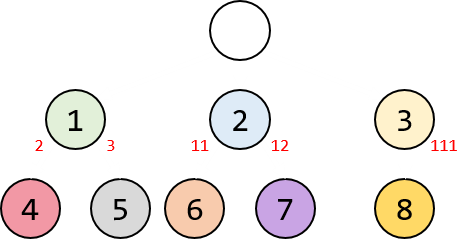
\includegraphics[width=0.3\textwidth]{images/WLLT}\\
	Master Thesis Seminar Talk	
}
%\title[MA Seminar Talk - Progress]{Master Thesis Seminar Talk}
%\titlegraphic{
%	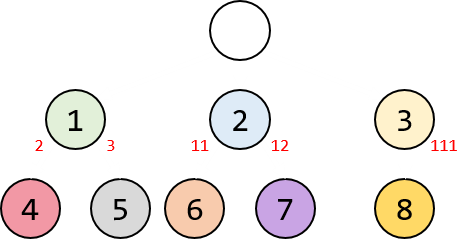
\includegraphics[width=0.2\textwidth]{images/WLLT}
%}
\subtitle{Progress Update}
\author[F. Beaumont]{Fabrice Beaumont}
\institute[]{Department of Information Systems and Artificial Intelligence - \textbf{Dr. Pascal Welke}}
\date{13. July 2022}

\newcommand{\figureWidth}{7cm}
\newcommand{\figureHorizontal}{2cm}
\newcommand{\figureVertical}{5cm}
\begin{document}


\begin{frame}
	\titlepage
\end{frame}

%%%%%%%%%%%%%%%%%%%%%%%%%%%%%%%%%%%%%%%%%%%%%%%%%%%%%%%%%%%%%%%%%%%%%%%%%
\section{Overview}

\begin{frame}
\frametitle{Recap} \vspace{-1cm}
	\begin{minipage}{0.45\textwidth}
		\textbf{RECAP PROGRESS}:\newline
		
		\textbf{May}:
		\begin{enumerate}
			\item Task formulation
			\item Dataset Loader module
			\newline
		\end{enumerate}
		
		\textbf{June}:
		\begin{enumerate}
			\item[1.] Wasserstein Distance
			\item[1.'] \textit{DataLoader:\\Software -> script.}
			\item[2.] \textcolor{orange}{\enquote{Naive} feedback loop} \newline
		\end{enumerate}
	\end{minipage}
	\begin{minipage}{0.45\textwidth}
		\textbf{NEXT STEPS}:\newline
		
		\textbf{May}:
		\begin{enumerate}
			\item Wasserstein Distance
			\item \enquote{Naive} feedback loop
			\newline
		\end{enumerate}
		
		\textbf{June}:
		\begin{enumerate}
			\item \enquote{Naive} feedback loop.
			\item Investigate its performance (and measures for it)
			\newline
			\item[]
		\end{enumerate}		
	\end{minipage}
\end{frame}

%%%%%%%%%%%%%%%%%%%%%%%%%%%%%%%%%%%%%%%%%%%%%%%%%%%%%%%%%%%%%%%%%%%%%%%%%

\begin{frame}
	\frametitle{Overview \& Outlook} \vspace{-1cm}
	\begin{minipage}{0.45\textwidth}
		\textbf{RECAP PROGRESS}:\newline
				
		\textbf{June}:
		\begin{enumerate}
			\item[1.] Wasserstein Distance
			\item[1.'] \textit{DataLoader:\\Software -> script.}
			\item[2.] \textcolor{orange}{\enquote{Naive} feedback loop} \newline
		\end{enumerate}
	
		\textbf{July} (Update for today):
		\begin{enumerate}
			\item Cleaning the datasets
			\item \textit{Preparing comparison}
			\item \textit{Rethinking the WLLT structure}
			\newline
		\end{enumerate}
	\end{minipage}
	\begin{minipage}{0.45\textwidth}
		\textbf{NEXT STEPS}:\newline		
		
		\textbf{June}:
		\begin{enumerate}
			\item \enquote{Naive} feedback loop.
			\item Investigate its performance (and measures for it)
			\newline
			\item[]
		\end{enumerate}		
		
		\textbf{July} (Outlook):
		\begin{enumerate}
			\item Finish the feedback loop
			\item Different edge weight trainings
			\item Edge weights via FRM
			\newline
		\end{enumerate}
	\end{minipage}
\end{frame}

%%%%%%%%%%%%%%%%%%%%%%%%%%%%%%%%%%%%%%%%%%%%%%%%%%%%%%%%%%%%%%%%%%%%%%%%%
\section{Some results}

\begin{frame}
\frametitle{New WLLT structure}
	For the computation of the WLLT I now use for files:
	\begin{itemize}
		\item Meta data (file names, wl-depth, nr. of tree vertices) \newline
		\item Tree data in form of \textbf{path lists} \newline
		\item Vertex labels of the \textbf{whole dataset} (\textbf{Vector}) \newline
		\item Edge weights (\textbf{Vector})
	\end{itemize}
\end{frame}

\begin{frame}
\frametitle{New WLLT structure}
	For the edge weight update:
	\begin{itemize}
		\item WLLT
		\item \textit{Chose between different update mechanism}
		\item \textbf{Tree-Wasserstein distances}\\
		\tiny{[2019, Tam Le, Tree-Sliced Variants of Wasserstein Distances]} \newline
	\end{itemize}

	For the evaluation:
	\begin{itemize}
		\item Cluster measures (max intra, min inter) (\textbf{Learning feedback})
		\item Classification accuracy compared to other methods
	\end{itemize}
\end{frame}

\begin{frame}
	\frametitle{Preparation of the performance comparison}	
	\begin{figure}
		\centering
		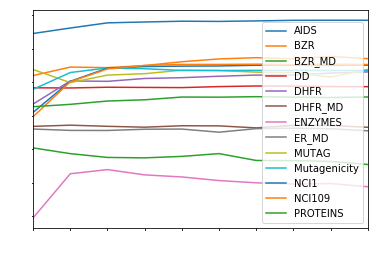
\includegraphics[width=0.6\linewidth]{images/plot_whiteText}
		\caption{Classification accuracies on databases using Weisfeiler-Lehman.}
		\label{fig:plot}
	\end{figure}
	\tiny{\texttt{grakel.kernels.\textbf{WeisfeilerLehman}(n\_iter=[1-10], base=grakel.kernels.VertexHistogram, normalize=True)}}\\
	\tiny{\texttt{grakel.utils.\textbf{cross\_validate\_Kfold\_SVM}(K, y, n\_iter=10)}}
\end{frame}

%%%%%%%%%%%%%%%%%%%%%%%%%%%%%%%%%%%%%%%%%%%%%%%%%%%%%%%%%%%%%%%%%%%%%%%%%
\section{End}

\begin{frame}[c]
	\centering %\Huge
	\begin{huge}
		\emph{Thank you all for listening.}\\
	\end{huge}
	\vspace{2 cm}
	I will be happy to answer any \textbf{questions} and\\
	hear your \textbf{comments}.
\end{frame}

%%%%%%%%%%%%%%%%%%%%%%%%%%%%%%%%%%%%%%%%%%%%%%%%%%%%%%%%%%%%%%%%%%%%%%%%%
\appendix
\section{Appendix}

\begin{frame}[noframenumbering]
	\frametitle{Example of the whole procedure}
	\begin{tikzpicture}[remember picture, overlay]
	\node[right] at (current page.west) 
	{
		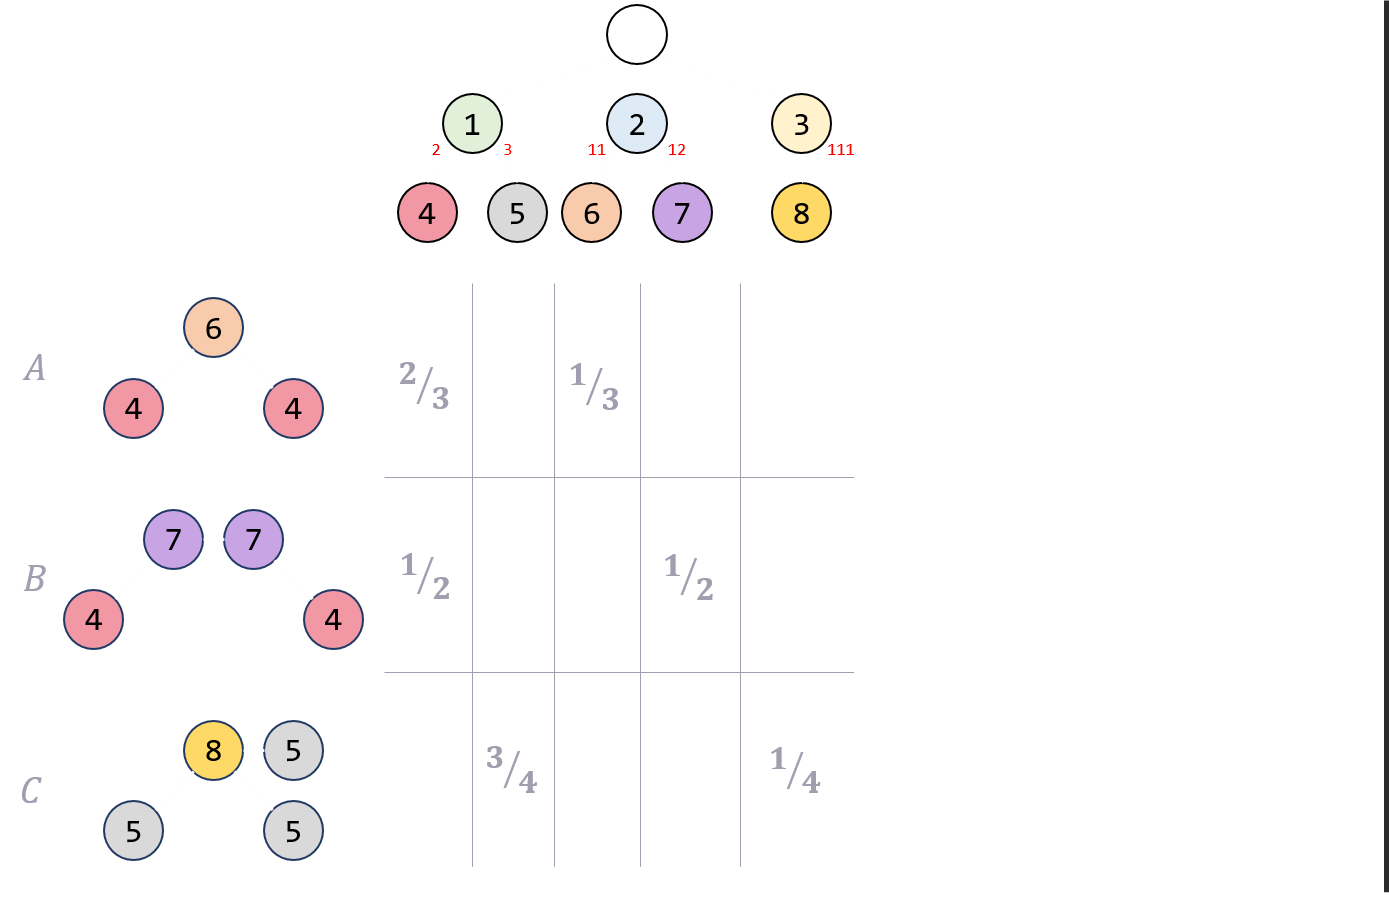
\includegraphics[width=0.9\textwidth]{images/Graphs7}
	};
	\end{tikzpicture}
	\begin{columns}[T]%beamer
		\column{0.7\textwidth}
		% blank
		\column{0.3\textwidth}
		\textbf{Tree metric}:\\
		$\begin{array}{ccccc}
		\ \ \; \textit{4} & \textit{5} & \textit{6} & \textit{7} & \textit{8}
		\end{array}$\\
		$
		\left(		
		\begin{array}{ccccc}
		\cdot & 2 & 4 & 4 & 4 \\
		& \cdot & 4 & 4 & 4 \\
		&   & \cdot & 2 & 4 \\
		& \upuparrows & & \cdot & 4\\
		&   &   &   & \cdot
		\end{array}
		\right)
		$\\
		\textbf{Wasserstein Dist.}:\\
		$\mathcal{W}_{t}(A,B) = \frac{4}{3}$\\
		$\mathcal{W}_{t}(A,C) = 3$\\
		$\mathcal{W}_{t}(B,C) = 3$\\
	\end{columns}
	\vspace{0.5cm}
	$d_{\text{WLLT}}(B,C) = 2*\frac{2}{4} + 4*\frac{1}{4} + 4*\frac{1}{4} = \frac{12}{4} = 3$
\end{frame}

\begin{frame}[noframenumbering]
	\frametitle{Example of the whole procedure}	
	\begin{columns}[T]%beamer
		\column{0.5\textwidth}
		\centering
		\textbf{Current clustering:}\\
		\vspace{0.5cm}
		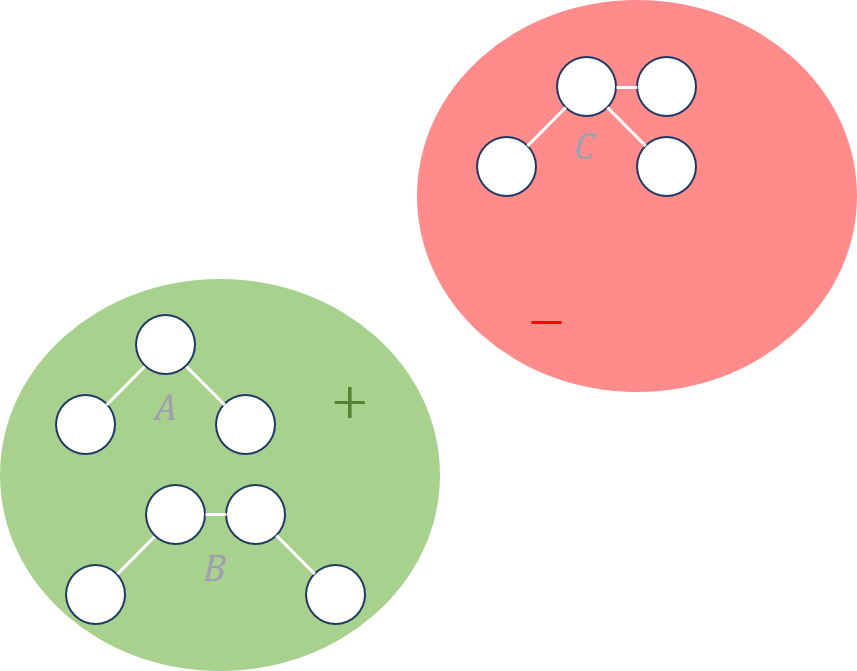
\includegraphics[width=0.8\textwidth]{images/Classification1}
		\column{0.5\textwidth}
		\centering
		\textbf{Target clustering:}\\
		\vspace{0.5cm}
		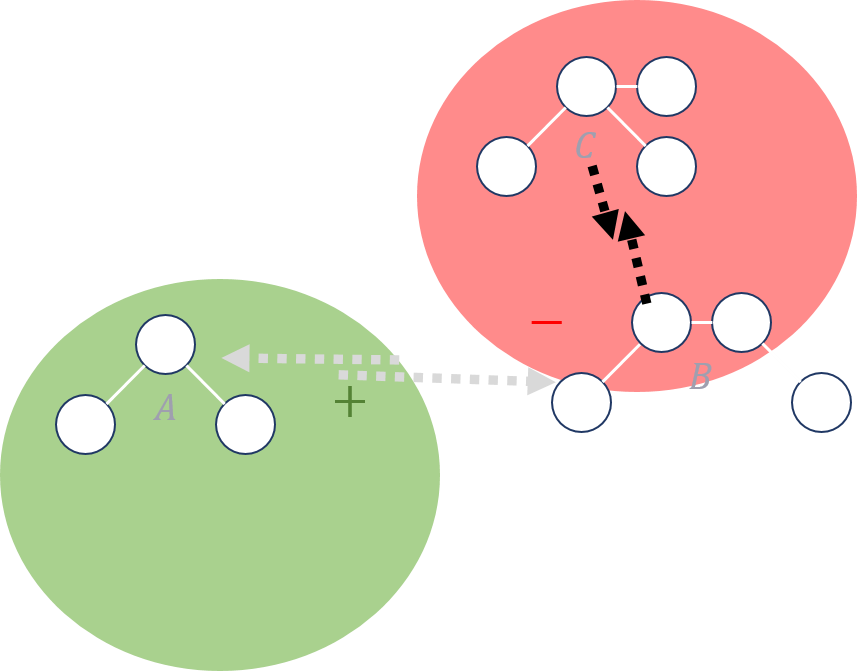
\includegraphics[width=0.8\textwidth]{images/Classification2}
	\end{columns}
	\vspace{0.5cm}
	Idea: Reduce distance between $B$ and $C$, by updating the edge weights.
\end{frame}

\begin{frame}[noframenumbering]
	\frametitle{Example of the whole procedure}	
	\begin{columns}[T]%beamer
		\column{0.5\textwidth}
		\centering		
		\textit{Local update} $P_{7,8}$:
		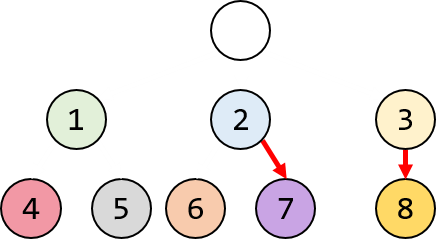
\includegraphics[width=0.8\textwidth]{images/WLLTUpdateEnds}
		\textit{Weighted path update} $P_{7,8}$:
		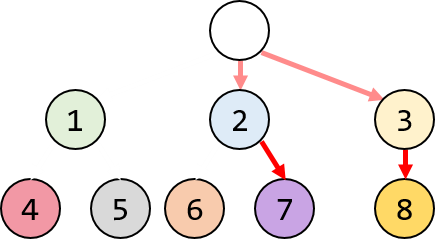
\includegraphics[width=0.8\textwidth]{images/WLLTUpdatePath}
		\column{0.5\textwidth}
		\begin{tikzpicture}[remember picture, overlay]
		\node[left] at (current page.east) [xshift=2.5cm, yshift=-0.5cm] 
		{
			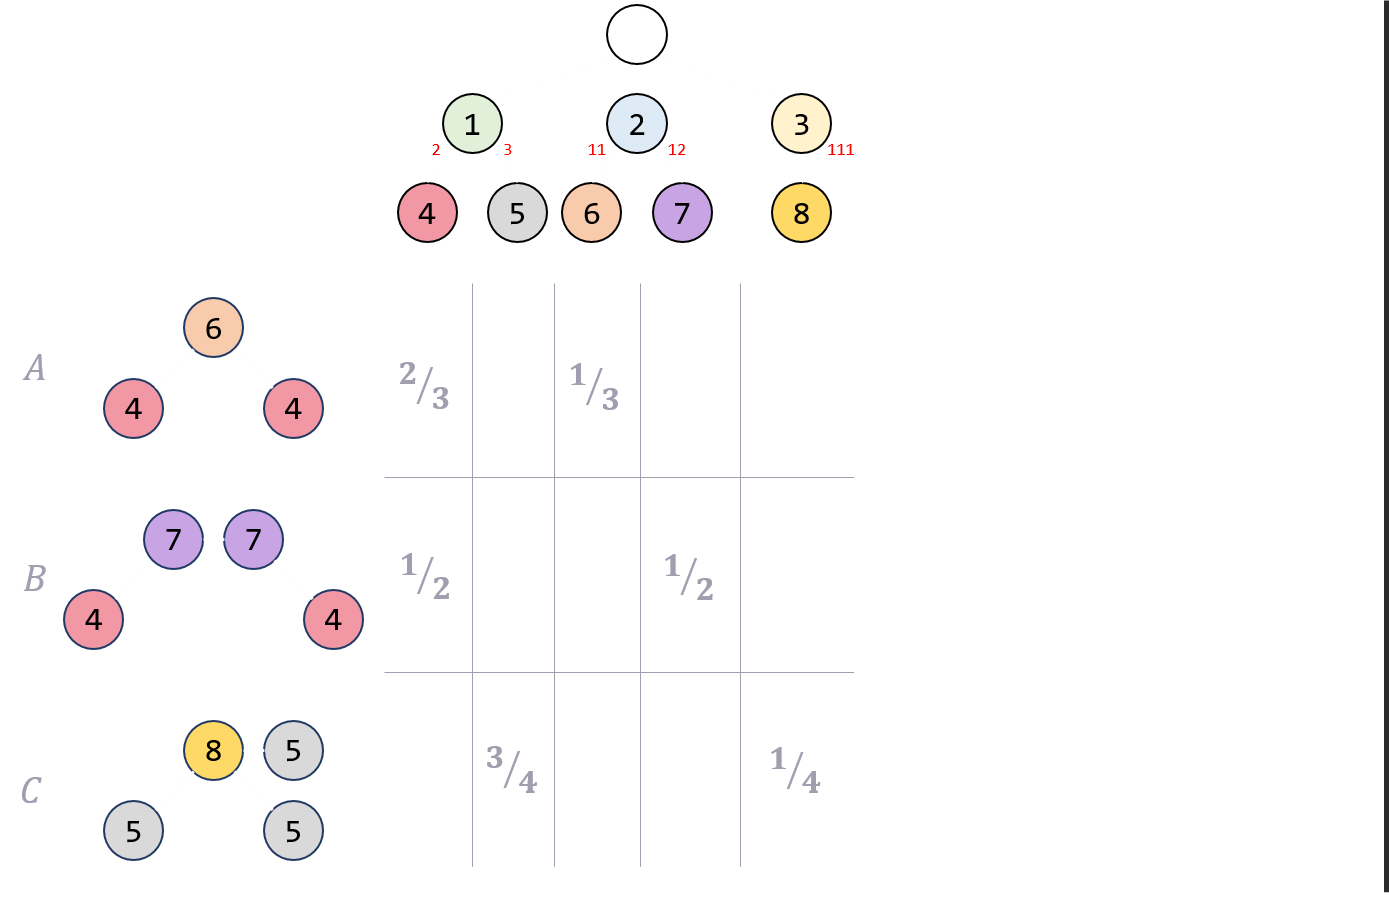
\includegraphics[width=1.2\textwidth]{images/Graphs7}
		};
		\end{tikzpicture}
	\end{columns}
\end{frame}

\begin{frame}[noframenumbering]
\frametitle{Implementation road-map 1/2}
\begin{itemize}
	\item \textbf{WLLT Construction}:
		\begin{itemize}
			\item Write to file and read from file. Construct WL-iteration based.
			\item All weights \textit{equal}.
			\item (\textit{Random} initial weights.)
			\item (Use \textit{a priori} knowledge.)
		\end{itemize}
	\item[]
	\item \textbf{Wasserstein-Distance feedback}:
		\begin{itemize}
			\item \enquote{Biggest pile of dirt}. 
			(\enquote{Smallest}, to increase the distance.)
			\item Distribution proportional to the pile size.
			\item Distribution proportional to the cost of moving the pile size.
		\end{itemize}	
\end{itemize}	
\end{frame}

\begin{frame}[noframenumbering]
\frametitle{Implementation road-map 2/2}
\begin{itemize}
	\item \textbf{Update rule}:
	\begin{itemize}
		\item Value:
		\begin{itemize}
			\item Constant $\lambda$.
			\item \textit{Gradient descent}.
		\end{itemize}
		\item Location:
		\begin{itemize}
			\item \textit{Local}: Only update the first and last edge weights of the connecting path.
			\item \textit{Weighted path}: Update all edge weights on the path, with less magnitude for edges closer to the root.
			\item \textit{Path}: Update all edges on the path.
			\item \textit{Global}: Update all edges, related to all occurring labels.
		\end{itemize}
	\end{itemize}		
\end{itemize}	
\end{frame}

\end{document}